
%----------------------------------------------------------------------------
\chapter{Preliminaries}
%----------------------------------------------------------------------------



\section{Modeling using graphs}

Structural and behavioral modeling of systems are often done using graphs, we use them for structural modeling of the system. Graphs are useful abstraction as they are easy to understand, and lots of algorithms can be used to process them.

\section{Runtime modeling}

In this thesis, we use structural modeling to model the current state of the system. This model is called the live model, which captures the state and the operating context of the system. We monitor the system through this model: The model is updated with sensor data and other information sources and the model itself is 

\subsection{Runtime modeling example}



\section{Graph pattern matching concepts}

\begin{figure}[h]
	\begin{center}
		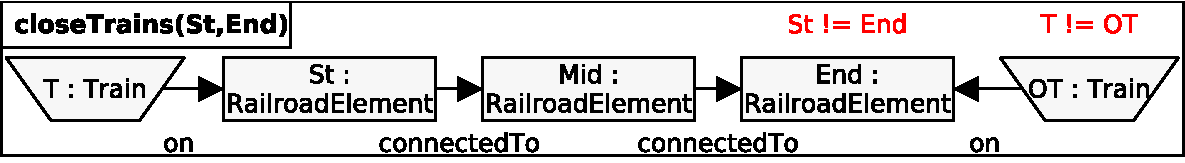
\includegraphics[width=0.75\textwidth]{figures/pattern-visual.pdf}
		\caption{Non-formal visual representation of a graph pattern}
		\label{pattern-visual}
	\end{center}
\end{figure}

A graph pattern's purpose is to define a set of constraints that can be satisfied by the vertices of the graph. A list of vertices satisfying those constraints is called a /emph{match}.

\section{Local search}

Local search~\cite{bur-marton-msc} is an algorithm to provide matchings of a graph pattern in a graph. It is a depth-first search in the space of variable bindings. In the root of the search tree all the variables are unbound. Then with each constraint, we add a new level for the tree. The child of a variable binding is all the other variable binding where 
\begin{itemize}
	\item The bound variables of the parent are bound to the same values as the corresponding variable in the child
	\item The constraint is satisfied by the child
\end{itemize}

The search tree can be traversed without materializing it with depth-first search. 

To optimize the size of the search tree the order of the constraints must be chosen 

\section{Distributed platform}

% adatok diszjunkt halmazokra bontva különböző csomópontra
% az algoritmusok is elosztottak, nem lesz összegyűjtve az infó, úgy van kiértékelve, hogy nincs aki mindent látna a rendszerből

Cyber-physical systems are distributed hence there are different ways to process the sensor data incoming into the computation nodes. \todo{különböző módok bemutatása mi diszjunk elosztott modellt választottunk}






